% This work is made available under the terms of the
% Creative Commons Attribution-ShareAlike 4.0 license,
% http://creativecommons.org/licenses/by-sa/4.0/.

\chapter{Machine learning}

\section{Dark Lord}
The \textit{Dark Lord} wizard allows you to set up and monitor a genetic
algorithm that determines the best set of attributes, based on the classifier
and metric you choose to optimize on. The output directory that you define
(see Figure \ref{darklord_setup}), is used to store all the \textit{reduced/optimized}
datasets that improved the metric and the classifier configurations. The following screenshots were obtained for
the \textit{triazines} regression dataset\footnote{\url{}{https://sourceforge.net/projects/weka/files/datasets/regression-datasets/regression-datasets.jar/download}}
using 1,000 iterations, notifications sent whenever a change occurs (``notificationInterval'' is 0)
and LinearRegression as classifier (with all attribute selection turned off).
The optimization can be paused, resumed or stopped with the buttons at the
bottom right of the view panel (see Figure \ref{darklord_run}).

\begin{figure}[htb]
  \centering
  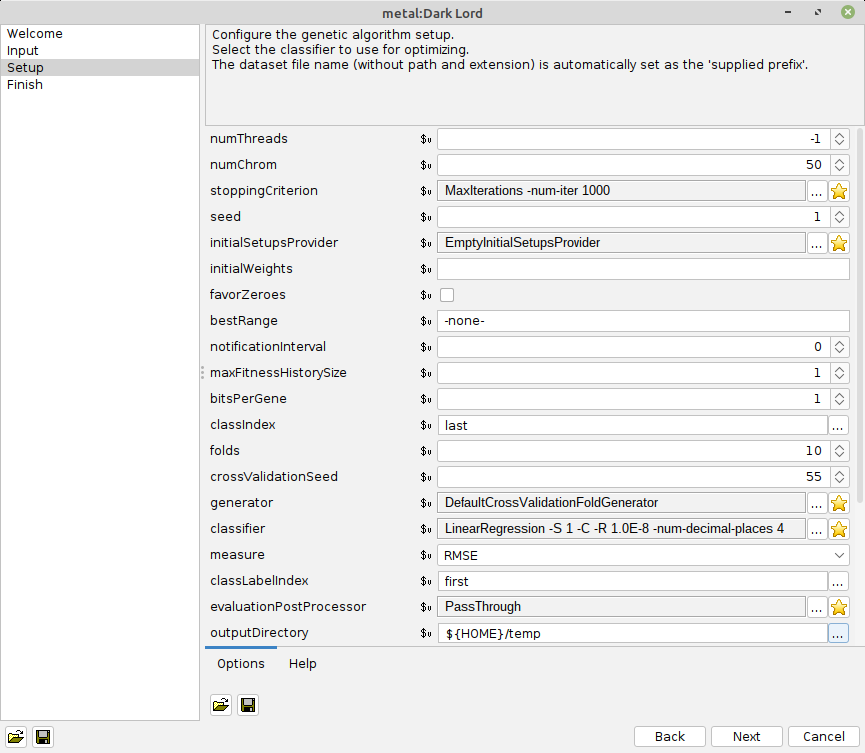
\includegraphics[width=12.0cm]{images/darklord_setup.png}
  \caption{Dark Lord setup.}
  \label{darklord_setup}
\end{figure}

\begin{figure}[htb]
  \centering
  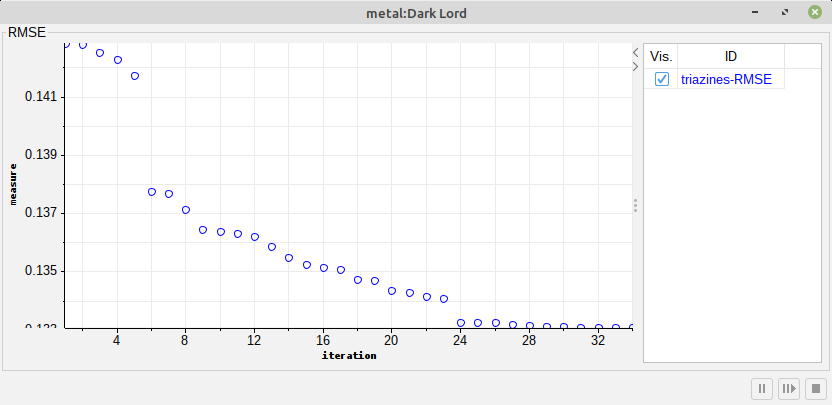
\includegraphics[width=12.0cm]{images/darklord_run.png}
  \caption{Dark Lord run.}
  \label{darklord_run}
\end{figure}

\clearpage
\section{Hermione}
The \textit{Hermione} wizard allows you to set up and monitor a genetic
algorithm that determines the best parameter settings, based on the classifier
and metric you choose to optimize on. The output directory that you define
(see Figure \ref{hermione_setup}), is used to store all the setups/datasets
that improved the metric. The optimization can be paused, resumed or
stopped with the buttons at the bottom right of the view panel (see Figure
\ref{hermione_run}). The screenshots were generated from optimizing
the GPD classifier's gamma/noise and the PLS filter's components (both wrapped
in a FilteredClassifier) on the \textit{triazines} regression
dataset\footnote{\url{}{https://sourceforge.net/projects/weka/files/datasets/regression-datasets/regression-datasets.jar/download}}.

\begin{figure}[htb]
  \centering
  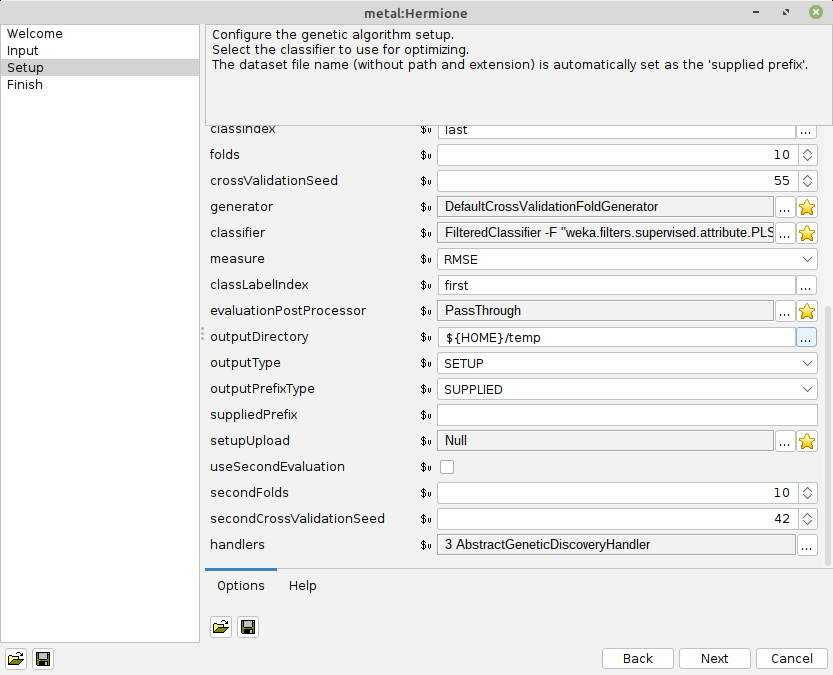
\includegraphics[width=12.0cm]{images/hermione_setup.png}
  \caption{Hermione setup.}
  \label{hermione_setup}
\end{figure}

\begin{figure}[htb]
  \centering
  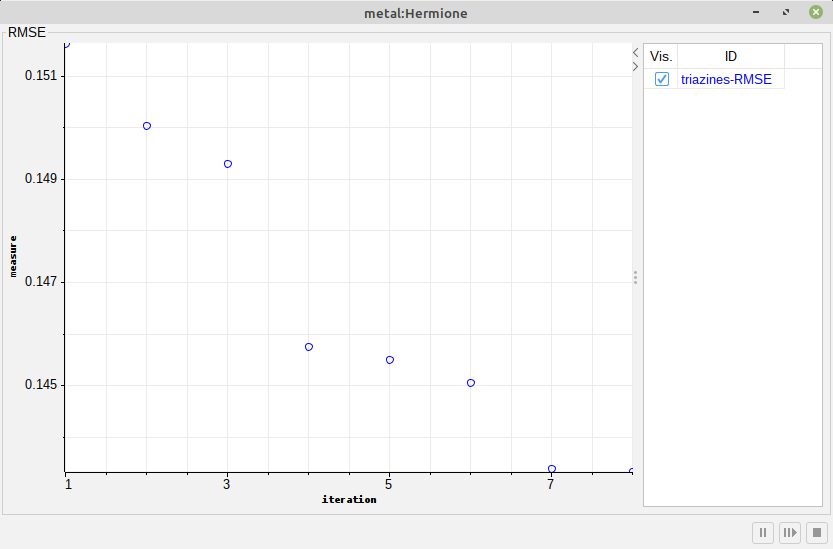
\includegraphics[width=10.0cm]{images/hermione_run.png}
  \caption{Hermione run.}
  \label{hermione_run}
\end{figure}

\clearpage
\section{WEKA Experimenter}
The classic interface of the \textit{WEKA Experimenter} is available in ADAMS as well.

\begin{figure}[htb]
  \centering
  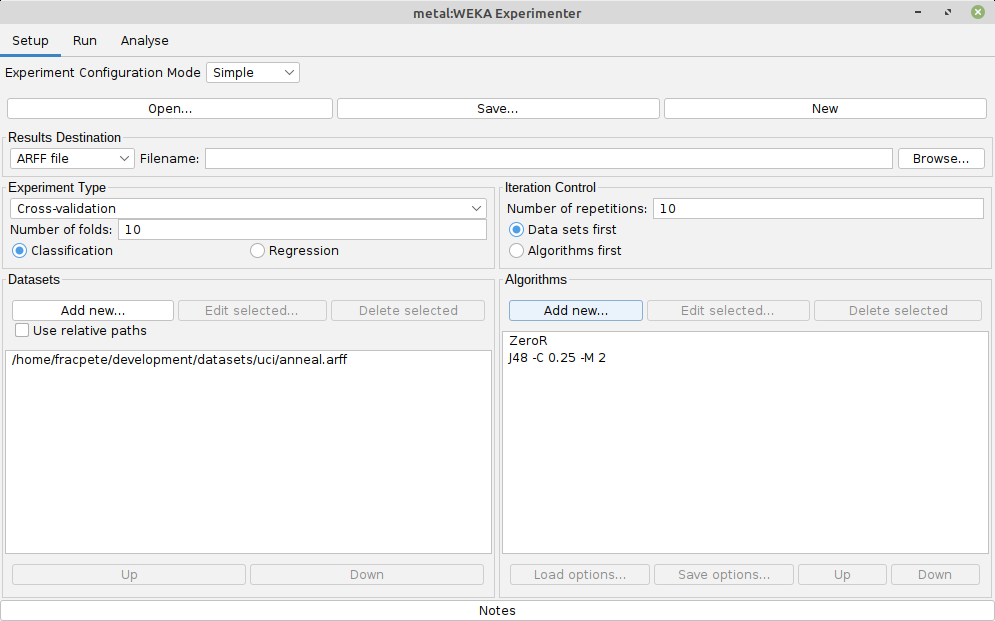
\includegraphics[width=12.0cm]{images/experimenter.png}
  \caption{Experimenter interface.}
  \label{experimenter}
\end{figure}

\clearpage
\section{WEKA Explorer}
The classic interface of the \textit{WEKA Explorer} is available in ADAMS as well.

\begin{figure}[htb]
  \centering
  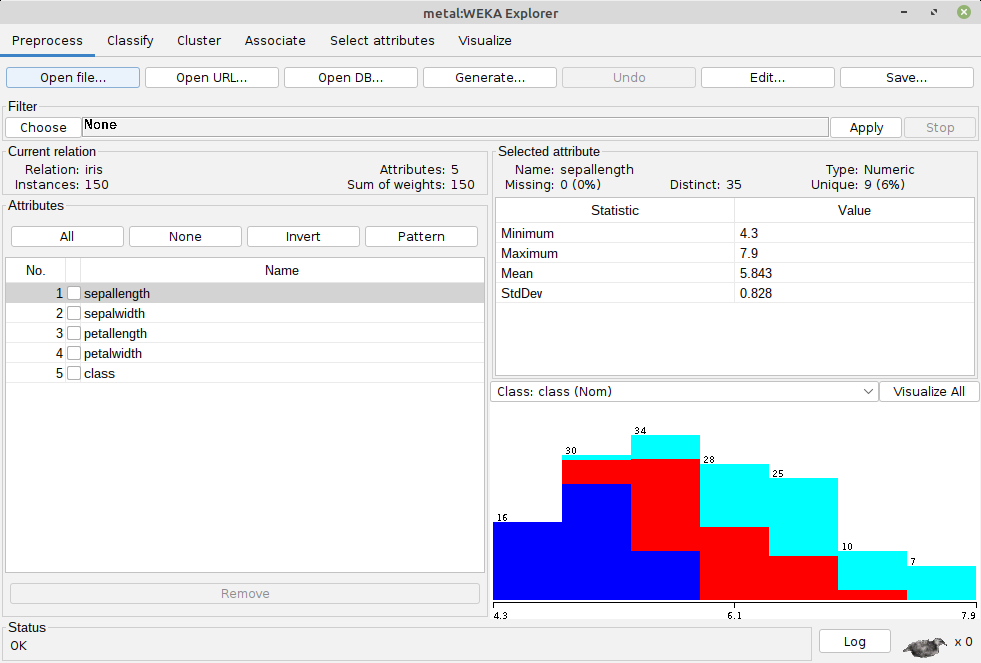
\includegraphics[width=12.0cm]{images/explorer.png}
  \caption{Explorer interface.}
  \label{explorer}
\end{figure}

\clearpage
\section{WEKA Investigator}
The \textit{WEKA Investigator} (see Figure \ref{wekainvestigator}) is aimed
to be a replacement of the WEKA Explorer. The idea is to have a more versatile
and efficient user interface: manage multiple sessions, each session can manage
multiple datasets (e.g., train and test set), making use of tabs instead of windows
(but output tabs can still be detached for comparison), configuration of
outputs to generate each time an evaluation is run (statistics, model,
classifier errors, etc).

\begin{figure}[htb]
  \centering
  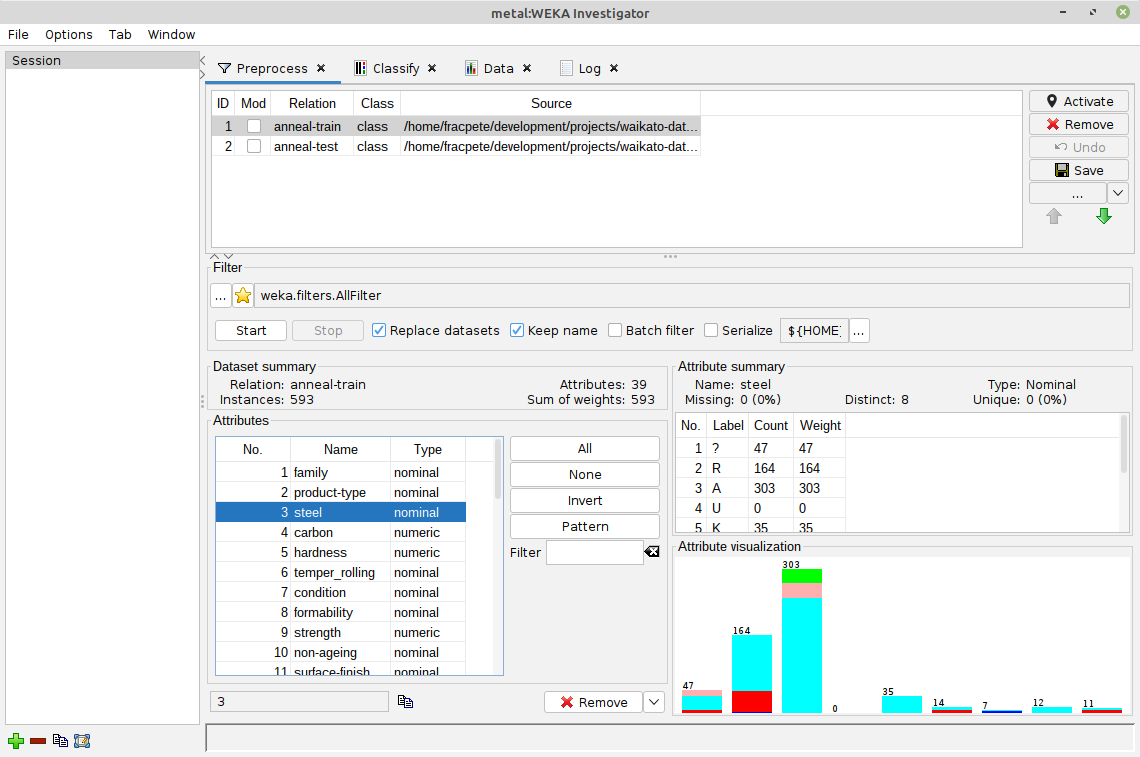
\includegraphics[width=12.0cm]{images/wekainvestigator.png}
  \caption{Weka Investigator.}
  \label{wekainvestigator}
\end{figure}

\clearpage
\section{WEKA Multi-Experimenter}
The \textit{Multi-Experimenter} interface allows multiple sessions within the same window,
as well as being able to run ADAMS or WEKA experiments. The statistical evaluation is
using WEKA's underlying API in both cases.

\begin{figure}[htb]
  \centering
  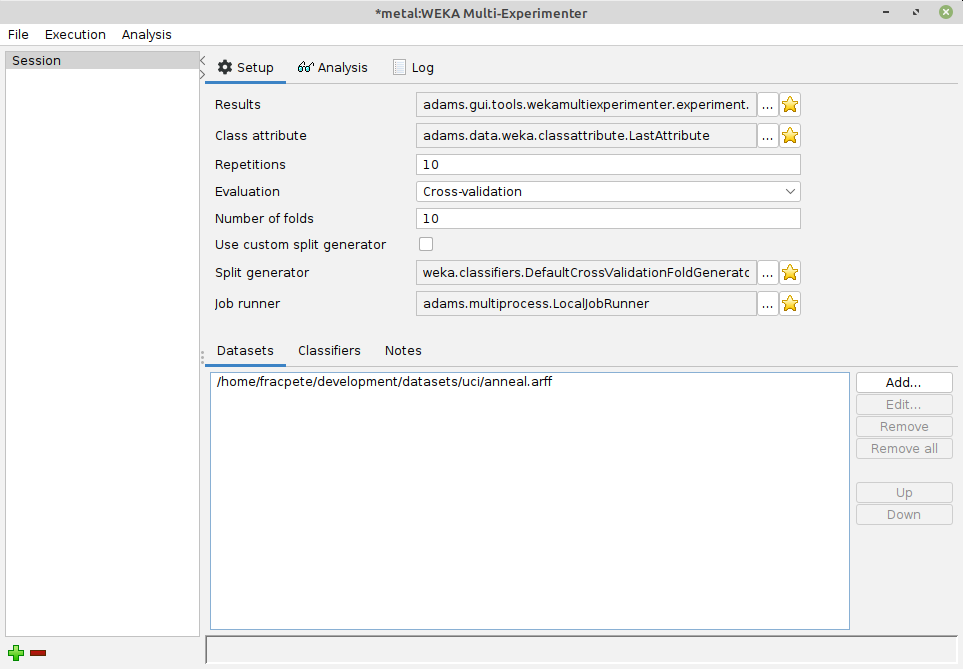
\includegraphics[width=12.0cm]{images/multi-experimenter.png}
  \caption{Multi-Experimenter.}
  \label{multi-experimenter}
\end{figure}

\clearpage
\section{WEKA Multi-Explorer}
ADAMS contains an extended version of the WEKA Explorer. The interface uses
menus instead of buttons to declutter the pre-process tab. Also, it keeps track
of the datasets that the user loads, to make re-loading recent files easier.
This saves a lot of time when working with the same files on a frequent basis.
Furthermore, the user can have an arbitrary number of Explorer sessions in the
same window, distinguished by names. Figure \ref{explorerext} shows the new
interface with the drop-down menu in action.

\begin{figure}[htb]
  \centering
  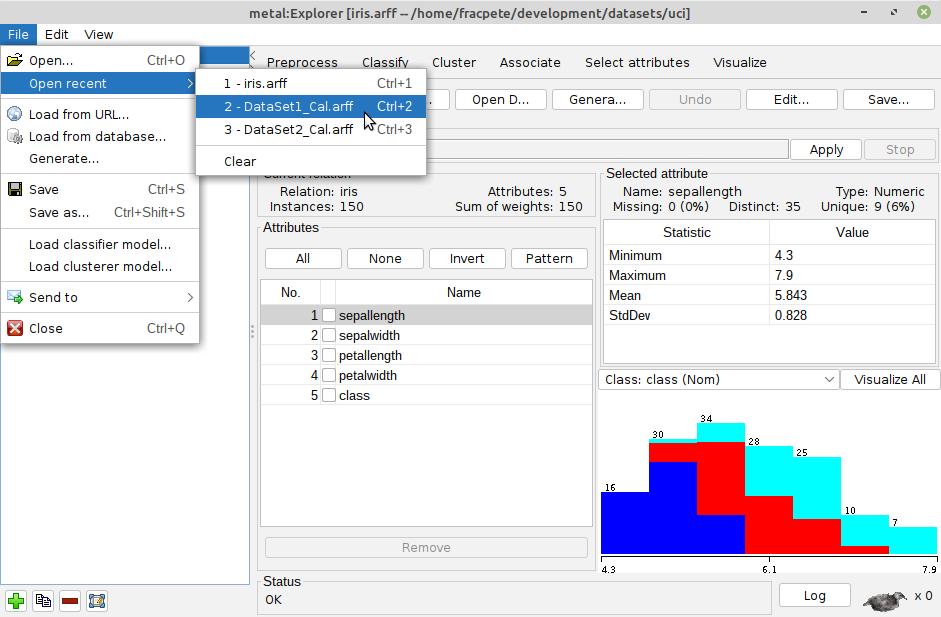
\includegraphics[width=12.0cm]{images/explorerext.png}
  \caption{Explorer interface with menus.}
  \label{explorerext}
\end{figure}

One very useful feature is the notion of \textit{workspaces} in this interface.
You can save the current setup (current dataset, classifiers, clusterers,
evaluation set up, results, etc.) to a file and restore all of it in one go
again. Unfortunately, not all data can be stored, such as the log, the undo
history and the built models or visualizations associated with a results.
See Figure \ref{explorerext-workspaces} for the button (highlighted in red)
that allows you to load/save workspaces.

\begin{figure}[htb]
  \centering
  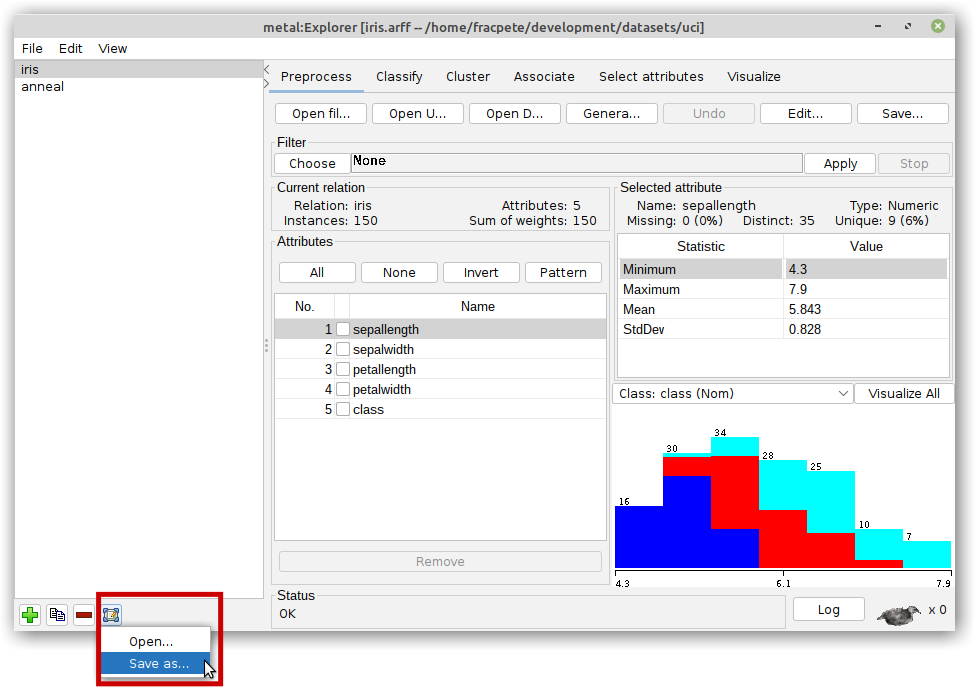
\includegraphics[width=12.0cm]{images/explorerext-workspaces.png}
  \caption{Saving/restoring of workspaces.}
  \label{explorerext-workspaces}
\end{figure}

\clearpage
\section{WEKA SimpleCLI}
Weka's basic command-line interface, \textit{SimpleCLI}, is also
available. A screenshot is shown in Figure \ref{simplecli}.

\begin{figure}[htb]
  \centering
  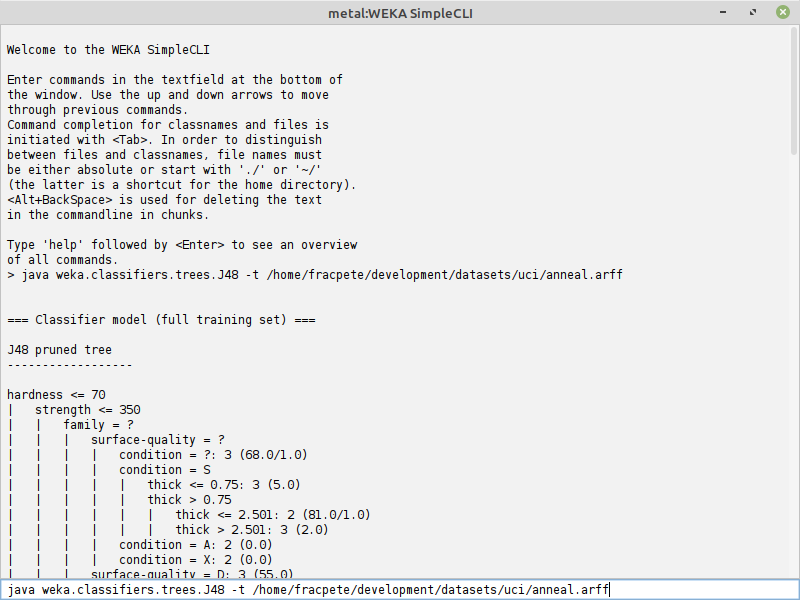
\includegraphics[width=12.0cm]{images/simplecli.png}
  \caption{The SimpleCLI interface.}
  \label{simplecli}
\end{figure}

\clearpage
\section{WEKA Workbench}
The more flexible alternative to the Explorer is called the \textit{Workbench}.
A screenshot is shown in Figure \ref{workbench}.

\begin{figure}[htb]
  \centering
  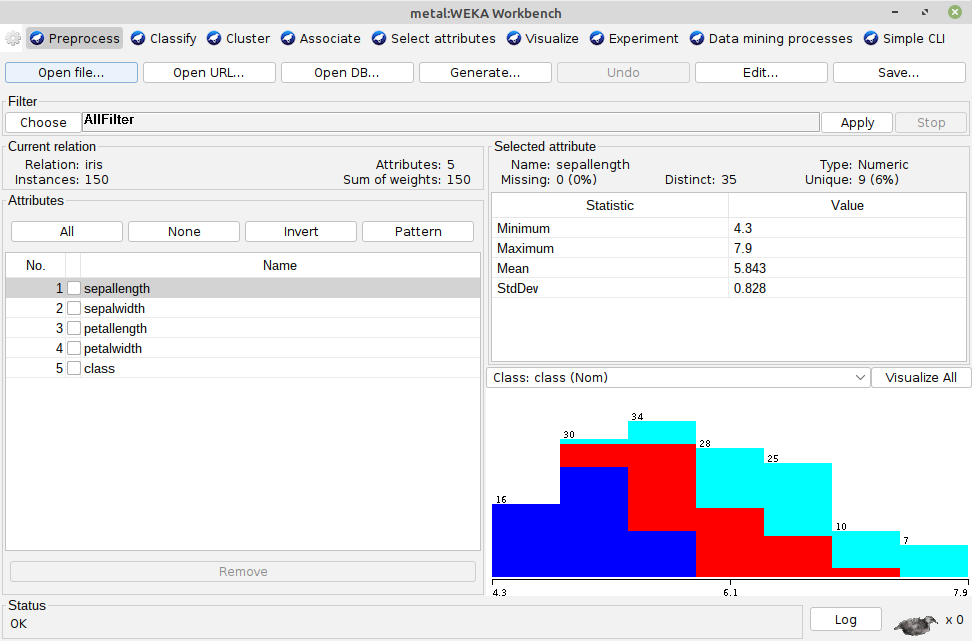
\includegraphics[width=12.0cm]{images/workbench.png}
  \caption{The Workbench interface.}
  \label{workbench}
\end{figure}
